\documentclass{article}
\usepackage[utf8]{inputenc}
\usepackage{setspace}
\usepackage[T1]{fontenc}

\usepackage{enumitem}
\usepackage{lmodern}
\usepackage{graphicx}


\usepackage{hyperref}
\hypersetup{
    colorlinks=true,
    linkcolor=blue,
    filecolor=magenta,      
    urlcolor=cyan,
    citecolor=red
}
 
\urlstyle{same}

\title{The Effects of Gross Foreign Direct Investment on the Growth Rate of High-Income Countries in the 21\textsuperscript{st} Century\\
\large Observational Studies - Midterm Summary Report}
\author{Chris Hayduk}
\date{\today}

\begin{document}
%\linespread{1.5}

\doublespacing

\maketitle

\section{Introduction \& Research Questions}
\quad The national government for each sovereign country usually focuses its efforts on broad goals, such as improving the education-level of the populace or strengthening national security. Economic growth is perhaps the most important of these goals, as a strengthening economy usually leads to higher wages and an improved standard of living for a country's population. One of the most common and well-known measures of economic strength is annual Gross Domestic Product (GDP), which measures the value of all goods and services produced in a country within a given year. GDP per capita divides this value by the country's total population, thus providing us with a proxy for the average wealth (and thus standard of living) in a country.\\
\null\quad There are many factors that contribute towards GDP per capita growth. This paper will specifically examine the effects of gross foreign direct investment (FDI) on a country's GDP per capita. The dichotomy between isolationist and globalist economic principles has become very pronounced over the last few years, especially in traditionally high income countries such as France, the United Kingdom, and the United States. These heated elections in various world powers have brought FDI to the forefront of national and international debates.\\
\null\quad There have been quite a few papers examining the effects of foreign direct investment on the growth rate of developing countries \cite{borensztein, hansen}. These papers contend that developing countries are able to benefit from the improved business practices and advanced technology provided by higher income countries \cite{borensztein}. However, this effect does not apply when limiting the scope of our analysis to the effects of FDI in high income countries, since they already possess a high level of technological advancement and business sophistication. Due to the heated discourse surrounding globalist economic principles and the lack of studies in this area, I will be focusing on gross FDI's impact on the growth rate of GDP per capita solely in high income countries in this paper.
%%%%%%%%%%%%%%%%%%%%%%%%%%%%%%%%%%%%%%
\section{Data Sources}
\quad Data on Gross Foreign Direct Investment was obtained from the OECD \href{https://data.oecd.org/}{website.} The data is labeled as "FDI stocks" and measures the total amount of foreign direct investment in a given year. The OECD website provides the option to download FDI stocks measured in US dollars or as a percent of the country's GDP. In order to control for varying economy sizes, I chose to download FDI stocks as a percent of the country's GDP. The data is available for the years 2005-2017, which is fine for the purposes of this paper, as I intend to focus on data from the 21\textsuperscript{st} century.\\
\null\quad Data on GDP per capita can be found on The World Bank's Open Data \href{https://data.worldbank.org/}{website.} The data ranges from 1960-2017. However, since the FDI data does not begin until 2005, I omitted all GDP per capita data prior to 2005. The World Bank Data also includes income classifications for each country, which fall into the following categories:
\begin{itemize}[noitemsep]
    \item High income
    \item Upper middle income
    \item Lower middle income
    \item Low income
\end{itemize}
This allowed me to easily separate high income countries from the rest of the data.\\
\null\quad In order to account for differences in technological level, I downloaded data from The World Bank regarding the number of scientific and technical journal articles published in each country per year. The fields considered for these articles are: physics, biology, chemistry, mathematics, clinical medicine, biomedical research, engineering and technology, and earth and space sciences. The data is available from 1970-2016. As in the case of the GDP per capita data, I omitted all data prior to 2005.
%%%%%%%%%%%%%%%%%%%%%%%%%%%%%%%%%%%%%%
\section{Methods}
\quad Before starting the modeling process, I needed to perform some data pre-processing in order to prepare it for regression. I began by taking the log of GDP per capita in 2005 and GDP per capita in 2017. This made the relationships between these two variables and the other predictors much more linear. I then took the difference of these two new variables, resulting in the change in log(GDP per Capita) from 2005 to 2017. This was then used as the predictor variable for the model.\\
\null\quad The Gross Foreign Direct Investment data was presented as a time series for each country from 2005-2017. In order to prepare the variable for input to a multiple regression model, I took the mean over this time period for each country. The number of journal articles per country presented a similar challenge, as it was also a time series from 2005-2016 for each country. For this variable, I took the mean over this period for each country. In addition, I divided the mean number of journal articles by the population (in 100 thousands) of each country. This resulted in the mean number of journal articles per 100,000 inhabitants for each country, allowing me to control for the differences in technological level without including any implicit data for the size of the country or its economy.\\
\null\quad I have included a table below with summary statistics for each variable included in the regression:
\begin{table}[!htbp] \centering 
  \caption{} 
  \label{} 
\begin{tabular}{@{\extracolsep{5pt}}lccccccc} 
\\[-1.8ex]\hline 
\hline \\[-1.8ex] 
Statistic & \multicolumn{1}{c}{N} & \multicolumn{1}{c}{Mean} & \multicolumn{1}{c}{St. Dev.} & \multicolumn{1}{c}{Min} & \multicolumn{1}{c}{Max} \\ 
\hline \\[-1.8ex] 
GDP per Capita in 2005 & 35 & 30,704.650 & 18,572.670 & 5,076.884 & 80,289.700 \\ 
GDP per Capita in 2017 & 35 & 39,709.230 & 22,132.970 & 13,863.180 & 104,103.000 \\ 
Mean FDI & 35 & 56.030 & 55.325 & 3.458 & 311.239 \\ 
Journal Articles per 100K Inhabitants & 35 & 122.237 & 54.994 & 17.401 & 243.698 \\ 
Log(GDP per Capita in 2005) & 35 & 10.111 & 0.728 & 8.532 & 11.293 \\ 
Log(GDP per Capita in 2017) & 35 & 10.434 & 0.577 & 9.537 & 11.553 \\ 
Change in Log(GDP per Capita) & 35 & 0.323 & 0.259 & $-$0.192 & 1.042 \\ 
\hline \\[-1.8ex] 
\end{tabular} 
\end{table}

I have also included a pairs plot in order to show the correlations between each pair of variables:
\begin{figure}	
	\centering
	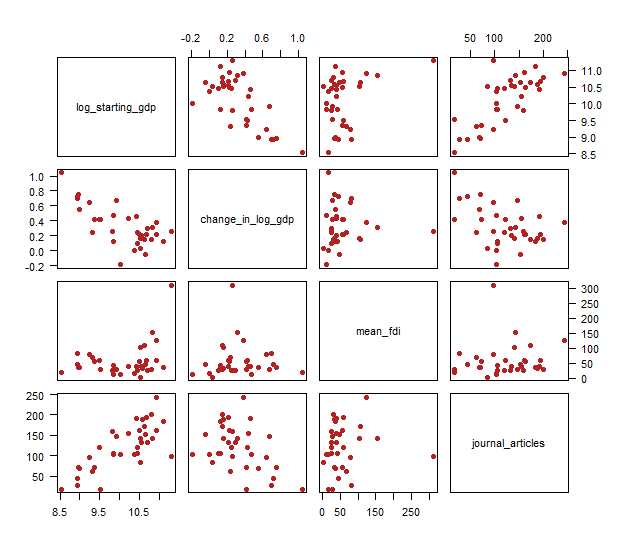
\includegraphics[width=\linewidth]{Rplot.png}
	\caption{Pairs plot of all variables included in the regression models.}
	\label{fig:pairs}
\end{figure}
\newpage
The regression models will now explore if mean Gross Foreign Direct Investment is a statistically significant predictor of the change in log(GDP per capita) for the period from 2005 to 2017 among high-income countries. I have decided to run three regressions. The first only explores the relationship between mean FDI and change in log(GDP per capita) without considering any covariates. The second model attempts to control for the differences in technological advancements between countries by including mean journal articles per 100K inhabitants. Lastly, the third model controls for differences in the starting wealth of each country's population by including log(GDP per capita in 2005) as a predictor. The results of these regressions are shown below:
\begin{table}[!htbp] \centering 
  \caption{Results} 
  \label{} 
\begin{tabular}{@{\extracolsep{5pt}}lccc} 
\\[-1.8ex]\hline 
\hline \\[-1.8ex] 
 & \multicolumn{3}{c}{\textit{Dependent variable:}} \\ 
\cline{2-4} 
\\[-1.8ex] & \multicolumn{3}{c}{change\_in\_log\_gdp} \\ 
\\[-1.8ex] & (1) & (2) & (3)\\ 
\hline \\[-1.8ex] 
 log\_starting\_gdp &  &  & $-$0.369$^{***}$ \\ 
  &  &  & (0.068) \\ 
  & & & \\ 
 mean\_fdi & 0.00000 & 0.0002 & 0.001$^{**}$ \\ 
  & (0.001) & (0.001) & (0.001) \\ 
  & & & \\ 
 journal\_articles\_per\_100k &  & $-$0.002$^{***}$ & 0.001$^{*}$ \\ 
  &  & (0.001) & (0.001) \\ 
  & & & \\ 
 Constant & 0.323$^{***}$ & 0.566$^{***}$ & 3.790$^{***}$ \\ 
  & (0.064) & (0.105) & (0.600) \\ 
  & & & \\ 
\hline \\[-1.8ex] 
Observations & 35 & 35 & 35 \\ 
R$^{2}$ & 0.00000 & 0.195 & 0.587 \\ 
Adjusted R$^{2}$ & $-$0.030 & 0.145 & 0.547 \\ 
Residual Std. Error & 0.262 (df = 33) & 0.239 (df = 32) & 0.174 (df = 31) \\ 
F Statistic & 0.00001 (df = 1; 33) & 3.884$^{**}$ (df = 2; 32) & 14.676$^{***}$ (df = 3; 31) \\ 
\hline 
\hline \\[-1.8ex] 
\textit{Note:}  & \multicolumn{3}{r}{$^{*}$p$<$0.1; $^{**}$p$<$0.05; $^{***}$p$<$0.01} \\ 
\end{tabular} 
\end{table} 
\newpage
%%%%%%%%%%%%%%%%%%%%%%%%%%%%%%%%%%%%%%
\section{Conclusion}
\quad We can see from the regression output that Gross Foreign Domestic Investment is not on its own a significant predictor of GDP per capita growth in high income countries in the 21\textsuperscript{st} century. It is also not significant when controlling for technological advancement. However, when controlling for both log(GDP per capita in 2005) and technological advancement, we see a small but significant (at the level $\alpha = 0.02$) positive effect from the mean gross foreign direct investment on the change in log(GDP per capita). As a result, we can conclude that, given a country with particular levels of individual wealth and technological advancement, an increased level of gross foreign direct investment will have a small positive effect on GDP per capita growth.
%%%%%%%%%%%%%%%%%%%%%%%%%%%%%%%%%%%%%%
\newpage
\begin{thebibliography}{9}
\bibitem{borensztein}
Eduardo Borensztein, Jose De Gregorio, Jong-Wha Lee.
\textit{How Does Foreign Direct Investment Affect Economic Growth?}. NBER Working Paper Series, March 1995.

\bibitem{hansen}
Henrik Hansen, John Rand.
\textit{On the Causal Links between FDI and Growth in Developing Countries}.
World Institute for Development Economics Research, June 2005.

\end{thebibliography}
\end{document}
